%        File: hw1.tex
%     Created: Sat Apr 06 10:00 AM 2013 P
% Last Change: Sat Apr 06 10:00 AM 2013 P
%
\documentclass[11pt]{article}

\usepackage{amsmath, amssymb, amsthm, cite, graphicx, float, mathrsfs, commath, dsfont, bbm, bm}
\usepackage[mathscr]{eucal}
\usepackage[sc]{mathpazo}
\linespread{1.05}
%\usepackage{setspace}
%\onehalfspacing
\usepackage[margin=1in, top=.8in, left=.8in]{geometry}
\usepackage{color}

% new commands
\DeclareMathOperator*{\argmin}{arg\,min}
\DeclareMathOperator*{\argmax}{arg\,max}
\DeclareMathOperator{\sgn}{sgn}
\newcommand{\E}{\mathrm{E}}
\newcommand{\Var}{\mathrm{Var}}
\newcommand{\Cov}{\mathrm{Cov}}
\newcommand{\Cor}{\mathrm{Cor}}
\newcommand{\id}{\operatorname{id}}
\newcommand{\diag}{\operatorname{diag}}
\newcommand{\Id}{\operatorname{Id}}
\newcommand{\tr}{\operatorname{tr}}
\newcommand{\Q}{\mathbb{Q}}
\newcommand{\C}{\mathbb{C}}
\newcommand{\R}{\mathbb{R}}
\newcommand{\Z}{\mathbb{Z}}
\newcommand{\F}{\mathbb{F}}
\newcommand{\N}{\mathbb{N}}

\newcommand{\indep}{\rotatebox[origin=c]{90}{$\models$}}

% 524 commands
%\newcommand{\norm}[1]{\| #1 \|}
\DeclareMathOperator{\spn}{span}
%\newcommand{\spn}{\operatorname{span}}
\newcommand{\onenorm}[1]{\| #1 \|_{L^1(\mathbb R^d)}}
\newcommand{\twonorm}[1]{\| #1 \|_{L^2(\mathbb R^d)}}

% 534 commands
\renewcommand{\Re}{\text{Re\,}}
\renewcommand{\Im}{\text{Im\,}}

\begin{document}
\pagestyle{empty}
\hfill Abraham Engle

\hfill Stat 571

\hfill \today
\begin{enumerate}
 	%1
	\item
		\begin{enumerate}
			\item The marginal mean is
			\begin{align*}
				E[Y_{ij}|X_{ij}=x] &= E[E[Y_{ij}|X_{ij}=x,b_i]] \\
				&= E[\mathrm{expit}(\beta_0 + b_i + \beta_1 x_{ij})] \\
				&= \mathrm{expit}(\beta_0 + \beta_1 x_{ij})\frac{1}{2} + \mathrm{expit}(\beta_0 -\beta_1 + \beta_1 x_{ij})\frac{1}{2}
			\end{align*}
			
			\item Assuming $\beta_0=0$, define
			\begin{align*}
				p_0 &= P(Y_{i0}=1|X_{i0}=x) = \frac{1}{2}(\mathrm{expit}(0) + \mathrm{expit}(-\beta_1)) \\
				p_1 &= P(Y_{i1}=1|X_{i1}=x) = \frac{1}{2}(\mathrm{expit}(0) + \mathrm{expit}(\beta_1))
			\end{align*}
			so $p_1=1-p_0$ since $\mathrm{expit}(z) = 1-\mathrm{expit}(-z)$. The likelihood for all $2n$ observations is
			\begin{align*}
				L(\beta_1) &= \prod_{i=1}^n p_0^{Y_{i0}}(1-p_0)^{1-Y_{i0}}p_1^{Y_{i1}}(1-p_1)^{1-Y_{i1}} \\
				&= \prod_{i=1}^n p_0^{Y_{i0}+1-Y_{i1}}(1-p_0)^{1-Y_{i0}+Y_{i1}},
			\end{align*}
			where $p_0 = p_0(\beta_1) = \frac{1}{2}(\frac{1}{2}+\mathrm{expit}(-\beta_1))$. The log-likelihood is
			\begin{align*}
				\ell(\beta_1) &= \sum_{i=1}^n [Y_{i0}+1-Y_{i1}]\log p_0 + [1-Y_{i0}+Y_{i1}]\log(1-p_0)
			\end{align*}
			with derivative
			\[
			 \od{\ell}{\beta_1} = \od{p_0}{\beta_1}\left( \sum_{i=1}^n \frac{1+Y_{i0}-Y_{i1}}{p_0} - \frac{1-Y_{i0}+Y_{i1}}{1-p_0} \right)
			\]
			Setting the quantity equal to zero and noting that the derivative $\od{p_0}{\beta_1} \neq 0$ for any value of $\beta_1$, we find that
			\[
				0 = \sum_{i=1}^n \frac{1+Y_{i0}-Y_{i1}}{p_0} - \frac{1-Y_{i0}+Y_{i1}}{1-p_0} \Longrightarrow \widetilde{p}_0 = \frac{1}{2} + \frac{1}{2n}\sum_{i=1}^n (Y_{i0}-Y_{i1})
			\]
			Since the maximizer $\widetilde{p}_0$ can be any real number in $[0,1]$ and we have the explicit contraints $p_0\in [1/4, 3/4]$, the quantity
			\[
				\max_{1/4\leq p_0\leq 3/4} \ell(p_0)
			\]
			is given by $\widetilde{p}_0$ provided it lies in the interval $[1/4, 3/4]$. If not, notice we have $\ell(p_0)$ increasing on $(0,\widetilde{p}_0)$ and decreasing on $(\widetilde{p}_0,1)$, so that
			\[
				\argmax_{1/4\leq p_0\leq 3/4} \ell(p_0) = \begin{cases}
					1/4 & \text{if } \widetilde{p_0}\leq 1/4 \\
					3/4 & \text{if } \widetilde{p_0} \geq 3/4 \\
					\widetilde{p}_0 & \text{otherwise.}
				\end{cases} = \begin{cases}
					1/4 & \text{if } \sum_{i=1}^n (Y_{i0}-Y_{i1}) \leq -n/2 \\
					3/4 & \text{if } \sum_{i=1}^n (Y_{i0}-Y_{i1}) \geq n/2 \\
					\widetilde{p}_0 & \text{otherwise.}
				\end{cases}
			\]
			From the earlier relationship that $p_0 = \frac{1}{4} + \frac{1}{2}\mathrm{expit}(-\beta_1)$, we have
			\[
				\widehat{\beta}_1:=\argmax_{\beta_1} \ell(\beta_1) = \begin{cases}
					\infty & \text{if } \sum_{i=1}^n (Y_{i0}-Y_{i1}) \leq -n/2 \\
					-\infty & \text{if } \sum_{i=1}^n (Y_{i0}-Y_{i1}) \geq n/2 \\
					-\mathrm{logit}(\frac{1}{2} + \frac{1}{n} \sum_{i=1}^n(Y_{i0}-Y_{i1})) & \text{otherwise.}
				\end{cases}
			\]
			\item Since the random variables $\{Y_{i0}\}$ are uncorrelated and have mean $E[Y_{i0}|X_{i0}=0] = p_0$ and similarly $\{Y_{i1}\}$ are uncorrelated with mean $p_1 = 1-p_0$, the law of large numbers gives
			\begin{align*}
				\frac{1}{n}\sum_{i=1}^n Y_{i0} &\to_p \frac{1}{2}(\mathrm{expit}(0) + \mathrm{expit}(-\beta_1)) \\
				\frac{1}{n}\sum_{i=1}^n Y_{i1} &\to_p \frac{1}{2}(\mathrm{expit}(0) + \mathrm{expit}(\beta_1)),
			\end{align*}
			so that
			\[
				\frac{1}{n}\sum_{i=1}^n (Y_{i0}-Y_{i1}) \to_p \frac{1}{2}(\mathrm{expit}(-\beta_1) - \mathrm{expit}(\beta_1)) = \begin{cases}
					-\frac{1}{2} & \text{if } \beta_1 = \infty \\
					\frac{1}{2} & \text{if } \beta_1 = -\infty \\
					(-\frac{1}{2}, \frac{1}{2}) & \text{if } |\beta_1| < \infty
				\end{cases}
			\]
			so as $n\to \infty$, by the rule for $\widehat{\beta}_1$ given above, we have
			\[
				\widehat{\beta}_1 \to_p \begin{cases}
					\infty & \text{when } \beta_1 = \infty \\
					-\infty & \text{when } \beta_1 = -\infty \\
					-\mathrm{logit}(\frac{1}{2} + \frac{1}{2}(\mathrm{expit}(-\beta_1) - \mathrm{expit}(\beta_1))) = \beta_1 & \text{otherwise},
				\end{cases}
			\]
			so $\widehat{\beta}_1$ is consistent. On the other hand, suppose the density on $b_i\sim H$ was mis-specified and free of $\beta_1$. We have
		\begin{align*}
			p_0 &= E[Y_{i0}|X_{i0}=0] = \int \mathrm{expit}(b_i)\dif H(b_i) \\
			p_1 &= E[Y_{i1}|X_{i1}=1] = \int \mathrm{expit}(b_i+\beta_1)(b_i)\dif H(b_i) = g(\beta_1)
		\end{align*}
		so using the MLE in (b), we have
		\[
			\frac{1}{n}\sum_{i=1}^n (Y_{i0}-Y_{i1}) \to_p p_0 - g(\beta_1).
		\]
		If the quantity $p_0-g(\beta_1)\in (-1/2,1/2)$, then in probability the MLE in (b) tends to
		\[
			-\mathrm{logit}(\frac{1}{2} +  p_0 - g(\beta_1)),
		\]
		which for arbitrary distributions $H$ will not reduce to $\beta_1$ as it did in the previous part, so we do not have consistency for $\beta_1$ in the misspecified case.
		\end{enumerate}
	%2
	\item
		\begin{enumerate}
			\item The contingency table is on 3.126. For this particular model, we have
			\begin{table}[H]
			\centering
				\begin{tabular}{c|cc|c}
				& $Y_{ij}=0$ & $Y_{ij}=1$ & Row Total \\
					\hline
					$j=0$ & 0/1 & 1/0 & 1\\
				$j=1$ & 0/1 & 1/0 & 1 \\
				\hline 
				Total & 0/2/1 & 2/0/1 & 2
				\end{tabular}
			\end{table}
			The row totals are always fixed to 1 since $Y_{ij}$ is binary-valued. The column totals can either be $(0,2), (2,0)$ or $(1,1)$ from the independence of the rows. By independence, the probabilities of observing a particular cell is (again following the format on 3.126)
			\begin{table}[H]
			\centering
				\begin{tabular}{c|cc|c}
				& $Y_{ij}=0$ & $Y_{ij}=1$ & Row Total \\
					\hline
					$j=0$ & $\frac{1}{1+\exp(\beta_0 + b_i)}$ & $\frac{1}{1+\exp(-(\beta_0 + b_i))}$ & 1\\
				$j=1$ & $\frac{1}{1+\exp(\beta_0 + b_i+\beta_1)}$ & $\frac{1}{1+\exp(-(\beta_0 + b_i+\beta_1))}$ & 1 \\
				\end{tabular}
			\end{table}
			Using this and the notation $C_{i0}$ and $C_{i1}$ to denote the column totals, the probabilities by independence are
			\begin{align*}
				P[C_{i0}=2, C_{i1}=0] &= \frac{1}{1+\exp(\beta_0 + b_i)}\times\frac{1}{1+\exp(\beta_0 + b_i+\beta_1)} \\
				P[C_{i0}=1, C_{i1}=1] &= \frac{1}{1+\exp(\beta_0 + b_i)}\times\frac{1}{1+\exp(-(\beta_0 + b_i+\beta_1))} \\				
				&+ \frac{1}{1+\exp(-(\beta_0 + b_i))}\times\frac{1}{1+\exp(\beta_0 + b_i+\beta_1)} \\
				P[C_{i0}=0, C_{i1}=2] &= \frac{1}{1+\exp(-(\beta_0 + b_i))}\times\frac{1}{1+\exp(-(\beta_0 + b_i+\beta_1))}
			\end{align*}
			\item Following the notation for LMM, we have $X_i = x = \begin{pmatrix}
				1 & 0 \\ 1 & 1
			\end{pmatrix}$ and we have $Z_i = z = \bm{1}$ so that
			\[
				\bm{\mu}_i = \mathrm{expit}(\bm{x}\bm{\beta} + \bm{z}b_i + \bm{\epsilon}_i)
			\]
			In this notation, a term appearing in the conditional likelihood (as seen on 3.124) is
			\[
				\frac{\exp(\bm{Y}_i^T\bm{x}\bm{\beta})}{\sum_{\bm{Y}':\bm{Y}'^T\bm{z} = \bm{Y}_i^T\bm{z}}\exp(\bm{Y}_i^{'T}\bm{x}\bm{\beta})} = \frac{\exp(Y_{i0}\beta_0 + Y_{i1}(\beta_0+\beta_1))}{\sum_{\bm{Y}':Y'_{i0}+Y'_{i1}=Y_{i0}+Y_{i1}}\exp(Y'_{i0}\beta_0 + Y'_{i1}(\beta_0+\beta_1))} = \frac{\exp(Y_{i1}\beta_1)}{\sum_{\bm{Y}':Y'_{i0}+Y'_{i1}=Y_{i0}+Y_{i1}} \exp(Y'_{i1}\beta_1)}.
			\]
			In this case, just as in the slides, we end up conditioning on column totals from sufficiency. The conditional likelihood used for inference on $\beta_1$ is thus the product of the term above over all clusters:
			\[
				L_c(\beta_1) = \prod_{i=1}^n \frac{\exp(Y_{i1}\beta_1)}{\sum_{\bm{Y}':Y'_{i0}+Y'_{i1}=Y_{i0}+Y_{i1}} \exp(Y'_{i1}\beta_1)}
			\]
			We can decompose this product into three cases depending on the value of the sufficient statistic $Y_{i0}+Y_{i1}=\bm{Y}_i^T\bm{1} \in \{0,1,2\}$.
			The conditional likelihood is
			\begin{align*}
				L_c(\beta_1) &= \left(\prod_{i:Y_{i0}+Y_{i1}=0}1\right) \times \left(\prod_{i:Y_{i0}+Y_{i1}=2}\frac{\exp(\beta_1)}{\exp(\beta_1)}\right) \\
				&\times\left(\prod_{i:Y_{i0}=1,Y_{i1}=0}\frac{1}{\exp(\beta_1)+1}\right)\times\left(\prod_{i:Y_{i0}=0,Y_{i1}=1}\frac{\exp(\beta_1)}{\exp(\beta_1)+1}\right) \\
				&= \sigma(-\beta_1)^{n_{10}}\sigma(\beta_1)^{n_{01}} \\
				&= (1-\sigma(\beta_1))^{n_{10}}\sigma(\beta_1)^{n_{01}}
			\end{align*}
			\item Suppose $\beta_1=0$. Write $\sigma$ as $\mathrm{expit}$ and $z=\beta_0+b_i$ for ease of notation. The probability vector for the column sum $C_{i1}$ is
			\[
				P(C_{i1}) = [(1-\sigma(z))^2,2\sigma(z)(1-\sigma(z)), \sigma(z)^2]^T,
			\]
			or in terms of $t=\sigma(z)$, we have
			\[
				P(C_{i1}) = [(1-t)^2,2t(1-t),t^2],
			\]
			obviously this is just a curve (1-dimensional) within the unit simplex. The values of $t$ that can work depend on $\beta_0$ and the random variable $b_i$. Since $\sigma$ maps $\R$ into $(0,1)$, regardless of the distribution of $b_i$ and the value of $\beta_0$, we have bounds $0<t<1$, so the graph of possible points on the simplex for a single cluster is
			\begin{figure}[H]
				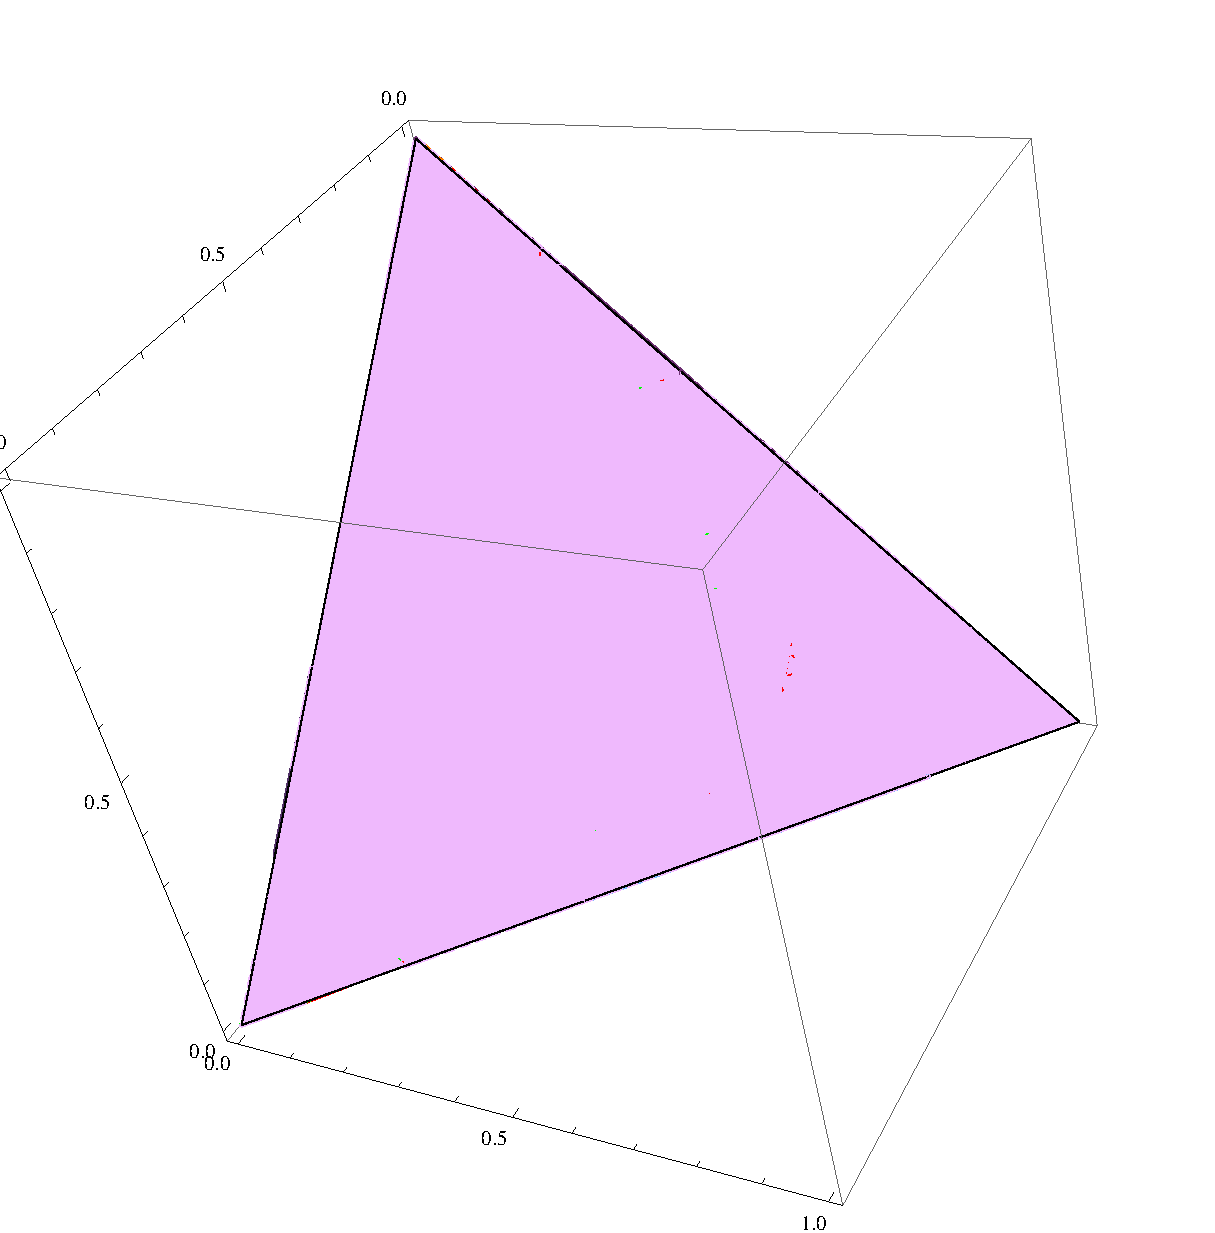
\includegraphics[scale=0.5]{plot1}
				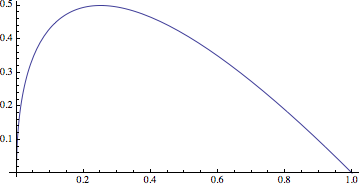
\includegraphics[scale=0.5]{projplot2c}
			\end{figure}
			where the second figure is a plot of the curve projected onto the $(x,y)$-plane, since the third component is completely determined by the first two. The second component of the probability vector is $2t(1-t)$, which cannot exceed $1/2$ for $0<t<1$ since $2t-2t^2$ is quadratic with its vertex (the maximum) at $t=1/2$, with value 1/2.
			\item Suppose $w=\beta_0+b_i\in \R$. The probability vector for $\beta_1=2$ is
			\[
				f(w):=P(C) = \begin{pmatrix}
				(1-\sigma(w))(1-\sigma(w+2)) \\
				\sigma(w)(1-\sigma(w+2)) + (1-\sigma(w))\sigma(w+2) \\
				\sigma(w)\sigma(w+2)
				\end{pmatrix}
			\]
			This is another curve living on the symplex, i.e., for any choice of $w\in \R$ (which implies freedom of choice of distribution for $b_i$ and value of $\beta_0$), we have $f(w) \in \Delta^2$. As $w$ varies over the real line, the curve $f(w)$ traces through an arc across the simplex. Plots similar to those in (c) are
			\begin{figure}[H]
				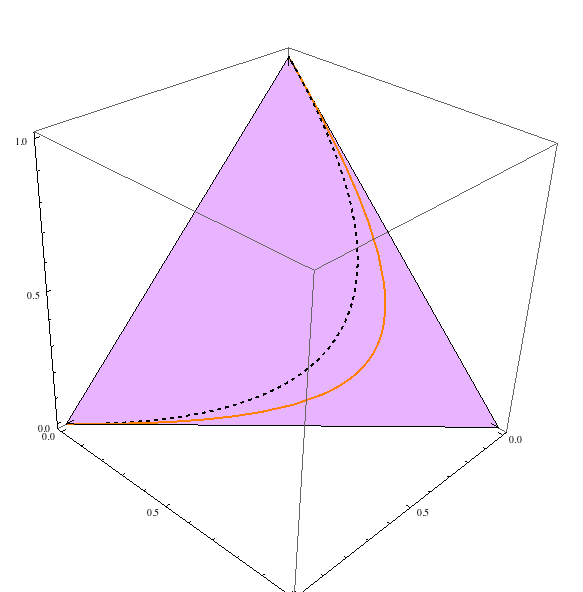
\includegraphics[scale=0.5]{plot2.png}
				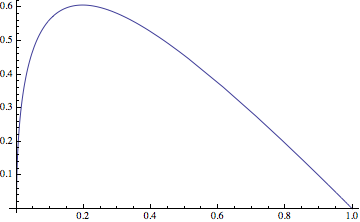
\includegraphics[scale=0.5]{projplot2d1}
				\caption{$\beta_1=2$ curve is thick, dashed curve is 2(c) for reference}
			\end{figure}	
			In similar fashion, we also have for $\beta_1=-2$,
			\begin{figure}[H]
				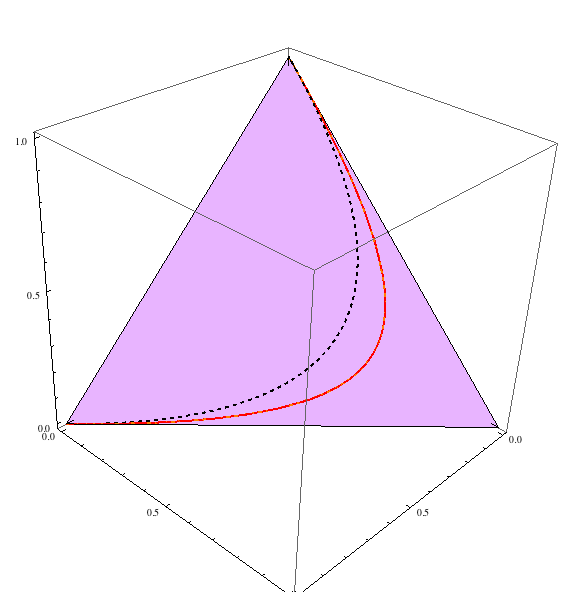
\includegraphics[scale=0.5]{plot3.png}
				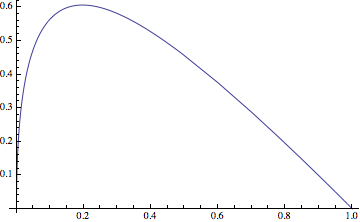
\includegraphics[scale=0.5]{projplot2d2}
				\caption{$\beta_1=-2$ curve is thick, dashed curves are the previous two for reference}
			\end{figure}	
			The curves appear to overlap for $\beta_1=\pm2$. For conditional likelihood inference, what this means is that we're specifying one of the possible curves that the probability vector can lie on. These curves do not appear to fill the simplex after I varied $\beta_1$ around, so this is not a very desirable property. 
			\item For conditional likelihood inference on $\beta_1$, we differentiate the logarithm of our formula at the end of (b), since the function $L_c$ is concave (which follows from the fact that $\log(1+e^{x})$ is convex):
			\[
				\od{\log(L_c)}{\beta_1} = \od{}{\beta_1} [n_{01}\log(\sigma(\beta_1)) + n_{10}\log(1-\sigma(\beta_1))] = n_{01}\frac{\sigma(\beta_1)\sigma(-\beta_1)}{\sigma(\beta_1)} + n_{10}\frac{-\sigma(\beta_1)\sigma(-\beta_1)}{\sigma(-\beta_1)},
			\]
			where we use the fact that $\sigma'(\beta_1)= \sigma(\beta_1)\sigma(-\beta_1))$. Thus we have
			\[
				\widehat{\beta}_1 = \mathrm{logit}\left(\frac{n_{01}}{n_{01}+n_{10}}\right) = \log\frac{n_{01}}{n_{10}}
			\]
			For the first data set, using GLMER in R and our formula above, we have
			\[
				\widehat{\beta}_0^{(MLE)}=-1.189, \widehat{\beta}_1^{(MLE)} = 1.193, \widehat{\sigma} = 1.393, \widehat{\beta}_1^{(cMLE)} = 1.306252
			\]
			For the second data set, we have
			\[
				\widehat{\beta}_0^{(MLE)}=-0.794, \widehat{\beta}_1^{(MLE)} = 1.376, \widehat{\sigma} = 0, \widehat{\beta}_1^{(cMLE)} = 1.306252
			\]
			The conditional MLEs are the same because the ratio of discordant pairs $n_{01}/n_{10}$ are the same in both data sets.
		\end{enumerate}
	%3
	\item
		\begin{enumerate}
			\item 
I generated data according to the hierarchical distribution $\beta_1 , b_i|\beta_1$ and apply sigmoids to obtain realizations $(\mu_{i0},\mu_{i1})$ and plot the implicit prior probabilities, shading by frequency:
			\begin{figure}[H]
			\centering
				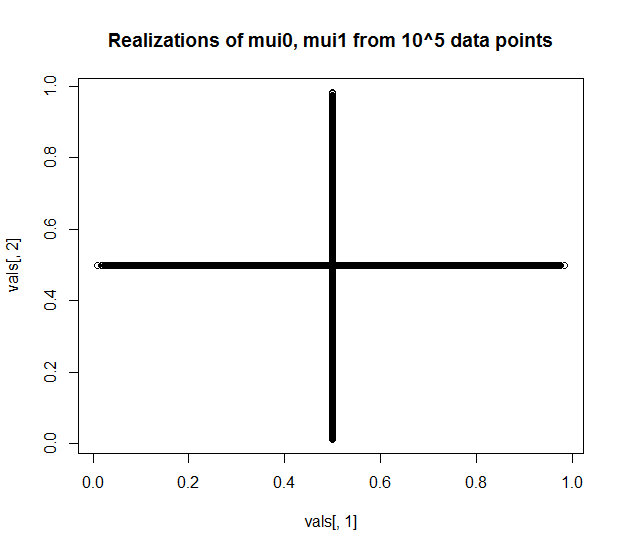
\includegraphics[scale=0.4]{Rplotp32}
			\end{figure}
			Since the empirical density appears to be symmetric about the line $y=x$, the parameters are exchangeable.
%b			
			\item 
			The joint density by independence is just the product of the marginal normal densities. If we define the transformation $T(b_i,\beta_1) = (y_1,y_2) = (\sigma(b_i),\sigma(b_i+\beta_1))$, then we have a $C^1$-diffeomorphism with inverse given by $(y_1,y_2)\mapsto (\mathrm{logit}(y_1),\mathrm{logit}(y_2)-\mathrm{logit}(y_1))$, so from Stat 512, we can find the density of the probabilities $\mu_{i0}, \mu_{i1}$ in terms of the determinant of the Jacobian matrix of this transformation. The matrix is triangular by the definition of the transformation, and I found
			\[
				\left|\pd{(bi,\beta_1)}{(y_1,y_2)}\right| = 					\frac{1}{y_1(1-y_1)y_2(1-y_2)},
			\]
			and thus the density of $(y_1,y_2)$ is
			\[
				f(y_1,y_2) = f((\mathrm{logit}(y_1),\mathrm{logit}(y_2)-\mathrm{logit}(y_1))\frac{1}{y_1(1-y_1)y_2(1-y_2)}\bm{1}_{(0,1)\times(0,1)}(y_1,y_2)
			\]
			Implementing this in R using the contour function, and simulations as done in (a), we have
			\begin{figure}[H]
				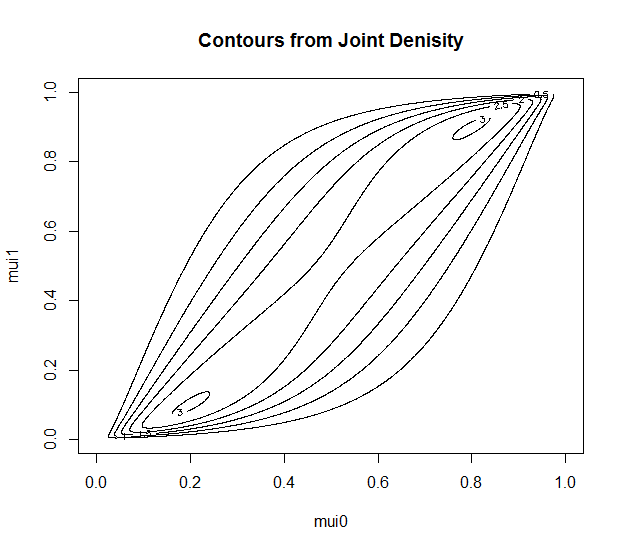
\includegraphics[scale=0.4]{Rplotp33}
				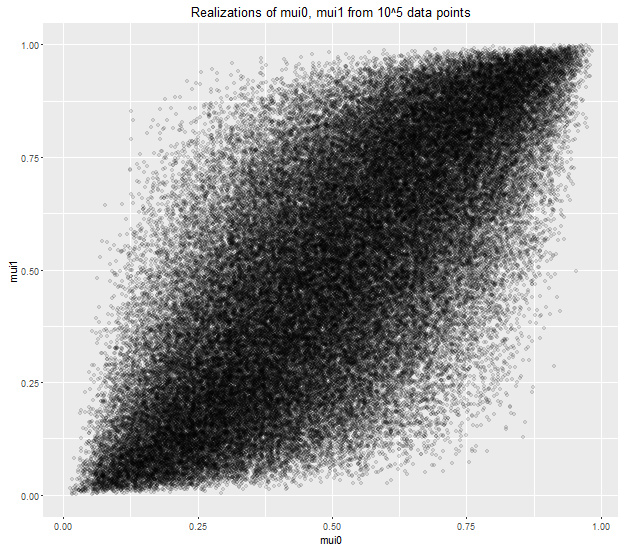
\includegraphics[scale=0.4]{Rplotp34}
			\end{figure}			
			In this case, the contours are not symmetric about the line $y=x$, so the parameters are not exchangeable.
		\end{enumerate}
	%4
	\item The slides 
		\begin{itemize}
			\item[Ch. 8]
				\begin{itemize}
					\item[\S 1,2]1.40-1.46
					\item[\S 3] Motivating dependent data modeling with efficiency, not really covered anywhere.
					\item[\S 4.]
						\begin{itemize}
							\item[1,2)] 3.23
							\item[3)] 3.8,9,10
						\end{itemize} 
					\item[\S 5] 3.11-3.13, 3.24-3.27, 3.37-3.44, 3.60-3.64
					\item[\S 6] 3.138-156 (methods), 3.157-185 (implementation). Didn't spend as much time discussing priors though.
					\item[\S 7] 2.4-2.6, 2.21-2.23, 2.40-2.48, 2.62-2.66 
					\item[\S 8] 2.75-2.99 (diagnostics and misspecification), 3.72-3.87 (diagnostics)
					\item[\S 9] Did not cover this example.
				\end{itemize}
			\item[Ch. 9]
				\begin{itemize}
					\item[\S 1,2] Motivation for link functions
					\item[\S 3] 3.89-3.94
					\item[\S 4] 3.95-3.107
					\item[\S 5] 3.121-3.135
					\item[\S 6] 3.138-156, 3.157-3.185. We did not separate the Bayes discussion.
					\item[\S 7] GLMM with Spatial dependence -- not really covered
					\item[\S 8] Conjugate Random Effects were mentioned briefly in class, but not in the notes I do not think.
					\item[\S 9] 2.38-2.42 and we read the paper by Liang for the midterm. We did not separate the discussion of GEE like the book does with LMM/GLMM and GEE using GLM.
					\item[\S 10] Do not think we discussed Connected GEE
					\item[\S 11] 3.101 for GLMM interpretation, 3.15 for differences, 2.152 for GEE interpretation using GLM
					\item[\S 12-14] We discussed binary outcomes as an example of GLM usage in GLMM and in GEE and in conditional likelihood approaches for GLMMs.
					\item[\S 15-19] 3.113 discusses some of the difficulties in nonlinearity obtaining marginal moments. Did not discuss much about the general theory/methods for NLMM though or any nonlinearity(non-link) in GEE.
					\item[\S 20] We discussed diagnostics in general for GEE with GLM, (G)LMM earlier, but did not discuss diagnostics of NLMM.
				\end{itemize}
		\end{itemize}
\end{enumerate}
\newpage
R Code
\begin{verbatim}
	m = 10^5
sigmoid <- function(x)
{
  return(1/(1+exp(-x)))
}
logit <- function(p)
{
  return( log(p/(1-p))
          )
}
vals = matrix(0,nrow=m,ncol=2)
vals2 = vals
x = c()
y = c()
for(i in 1:m)
{
  beta1 = rnorm(1)
  temp = rbinom(1,1,0.5)
  if(temp == 0)
    bi = 0
  else bi = -beta1
  bi2 = rnorm(1)
  x = append(x,beta1)
  y = append(y,bi)
  vals[i,1] = sigmoid(bi)
  vals[i,2] = sigmoid(bi+beta1)
  vals2[i,1] = sigmoid(bi2)
  vals2[i,2] = sigmoid(bi2+beta1)
}

joint <- function(b,beta1)
{
  if(b == 0 || b == -beta1)
  {
    ans = 0.5*dnorm(beta1)
  }
  else ans = 0
  ans
}

Jacobian <- function(mu0, mu1)
{
  return(
    1/(mu0-mu0^2) * 1/(mu1-mu1^2)
  )
}

mesh = 0.001
mu0 <- mu1 <- seq(0+mesh,1-mesh,by=mesh)
z <- matrix(0,nrow=length(mu0),ncol=length(mu0))
w <- z
for(i in 1:length(mu0))
{
  for(j in 1:length(mu0))
  {
    z[i,j] = joint(logit(mu0[i]),logit(mu1[j])-logit(mu0[i]))*Jacobian(mu0[i],mu1[j])
    w[i,j] = dnorm(logit(mu0[i]))*dnorm(logit(mu1[j])-logit(mu0[i]))*Jacobian(mu0[i],mu1[j])
  }
}


contour(mu0,mu1,z,main="Contours from Joint Denisity", xlab="mui0", ylab="mui1")
plot(vals[,1],vals[,2], main="Realizations of mui0, mui1 from 10^5 data points")
contour(mu0,mu1,w,main="Contours from Joint Denisity", xlab="mui0", ylab="mui1")
qplot(vals2[,1],vals2[,2], main="Realizations of mui0, mui1 from 10^5 data points",alpha=I(1/10),xlab="mui0", ylab="mui1")

setwd("~/Dropbox/UW2015-2016/Win2016/571/hw9")
library(lme4)
dat1 <- read.table("pairsdata1.txt", header=T)
dat2 <- read.table("pairsdata2.txt", header=T)
m1 <- glmer(y~x+(1|id), data=dat1, family=binomial)
m2 <- glmer(y~x+(1|id), data=dat2, family=binomial)

pair1 <- dat1[order(dat1$id,dat1$x),]
pair2 <- dat2[order(dat2$id,dat2$x),]

n01 <- sum(pair1$y[seq(1, nrow(pair1), 2)] == 0 & pair1$y[seq(2, nrow(pair1), 2)] == 1)
n10 <- sum(pair1$y[seq(1, nrow(pair1), 2)] == 1 & pair1$y[seq(2, nrow(pair1), 2)] == 0)
n00 <- sum(pair1$y[seq(1, nrow(pair1), 2)] == 0 & pair1$y[seq(2, nrow(pair1), 2)] == 0)
n11 <- sum(pair1$y[seq(1, nrow(pair1), 2)] == 1 & pair1$y[seq(2, nrow(pair1), 2)] == 1)

#first
cbeta1 <- log(n01/n10) #1.306252

n01 <- sum(pair2$y[seq(1, nrow(pair2), 2)] == 0 & pair2$y[seq(2, nrow(pair2), 2)] == 1)
n10 <- sum(pair2$y[seq(1, nrow(pair2), 2)] == 1 & pair2$y[seq(2, nrow(pair2), 2)] == 0)
n00 <- sum(pair2$y[seq(1, nrow(pair2), 2)] == 0 & pair2$y[seq(2, nrow(pair2), 2)] == 0)
n11 <- sum(pair2$y[seq(1, nrow(pair2), 2)] == 1 & pair2$y[seq(2, nrow(pair2), 2)] == 1)

cbeta1 <- log(n01/n10) #1.306252 both times

\end{verbatim}
\newpage
\begin{verbatim}
	
\end{verbatim}
\end{document}



